%(BEGIN_QUESTION)
% Copyright 2006, Tony R. Kuphaldt, released under the Creative Commons Attribution License (v 1.0)
% This means you may do almost anything with this work of mine, so long as you give me proper credit

Et trykkalibreringsinstrument kalt {\it deadweight tester} genererer svært presise trykk ved hjelp av kalibrerte vekter plassert på et hydraulisk stempel:

$$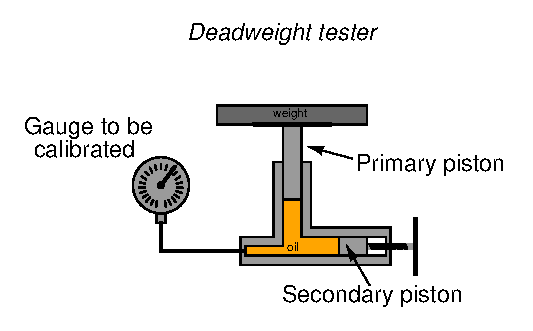
\includegraphics[width=15.5cm]{i00153x01.eps}$$

Sekundærstempelet beveges inn og ut ved å dreie et håndtak på en gjenget aksling. Den eneste oppgaven er å fortrenge nok olje til at primærstempelet løftes fra hvileposisjon slik at det bæres helt av oljetrykket. I denne tilstanden blir måleren utsatt for trykket som tilsvarer vektene på primærstempelet og arealet av primærstempelet.

Hva skjer med målerverdien hvis sekundærstempelet presses lenger inn? Hva skjer hvis sekundærstempelet trekkes ut, men ikke så langt at primærstempelet setter seg i hvileposisjon? Med andre ord: hvilken effekt har {\it posisjonen} til sekundærstempelet på trykket som påføres måleren?

$$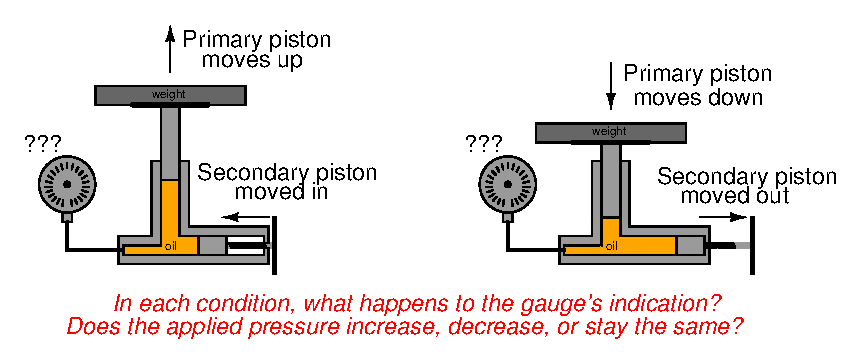
\includegraphics[width=15.5cm]{i00153x02.eps}$$

\vskip 20pt \vbox{\hrule \hbox{\strut \vrule{} {\bf Forslag til sokratisk diskusjon} \vrule} \hrule}

\begin{itemize}
\item{} Hvorfor regnes deadweight testere som nøyaktige {\it standarder} for fluidtrykk? Hvilke egenskaper i design/drift gir den høye nøyaktigheten? Omvendt: hva måtte endres for å forringe den innebygde nøyaktigheten?
\item{} Hvis en tekniker bytter væsketype i en deadweight tester (f.eks. fra én oljetype til en annen), endres nøyaktigheten?
\item{} Identifiser mulige problemer ved bruk av deadweight tester. Hva konkret kan gå galt med enheten?
\end{itemize}

\underbar{file i00153}
%(END_QUESTION)





%(BEGIN_ANSWER)

Ideelt sett vil sekundærstempelposisjonen ha {\it ingen effekt} på oljetrykket til måleren. Derfor skal målerverdien ikke endre seg.

%(END_ANSWER)





%(BEGIN_NOTES)

Så lenge primærstempelet er helt båret av oljetrykk, {\it må} oljetrykket være lik kraften fra vektene (som ikke endres) delt på arealet av primærstempelet (som heller ikke endres). Sekundærstempelet fortrenger bare olje for å løfte/senke primærstempelet. Det kan ikke «feilkalibrere» testeren så lenge primærstempelet ikke hviler mot noe som avlaster vekten og dermed reduserer oljetrykket. Med andre ord: utgangstrykket er enten korrekt eller klart feil, og det er lett å se når trykket ikke stemmer.

I praksis kontrolleres binding i primærstempelet ved å rotere det forsiktig mens sekundærstempelet presses inn. Når primærstempelet er helt båret av olje, skal det rotere fritt, og massen i kalibreringsvektene gir lang «frirull». Langsom rotasjon overkommer statisk friksjon og lar stempelet finne posisjonen med minst motstand.

Jeg anbefaler sterkt å ta med en faktisk deadweight tester i undervisning for live demonstrasjon, helst med en trykkmåler koblet til.

\vskip 10pt

En vanlig misforståelse blant studenter er at en deadweight tester måler trykk. Det stemmer ikke. En deadweight tester {\it genererer} presist kjente trykk for kalibrering av {\it andre} måleinstrumenter.

%INDEX% Calibration, deadweight tester: basic operation
%INDEX% Physics, static fluids: Pascal's Principle

%(END_NOTES)
